% EMERGE @ MICCAI 2026 poster for Paper-0018 (When Simple Wins).
% A0 portrait (841 x 1189 mm). Numbers are taken from the camera-ready
% WhenSimpleWins.tex; build with: latexmk -pdf poster.tex
\documentclass[25pt, a0paper, portrait, margin=0mm, innermargin=18mm,
  blockverticalspace=10mm, colspace=16mm, subcolspace=8mm]{tikzposter}

\usepackage[T1]{fontenc}
\usepackage{helvet}
\renewcommand{\familydefault}{\sfdefault}
\usepackage{amsmath}
\usepackage[eulergreek]{sansmath}
\sansmath
\usepackage{booktabs}
\usepackage{graphicx}
\usepackage{pgfplots}
\pgfplotsset{compat=1.18}
\usetikzlibrary{positioning}
\graphicspath{{../figures/}}

\definecolor{nuBlue}{HTML}{0B3D91}
\definecolor{nuRed}{HTML}{C8102E}
\definecolor{ink}{HTML}{1F2328}
\definecolor{paleBlue}{HTML}{EAF0FA}
\definecolor{vggC}{HTML}{0B3D91}
\definecolor{resC}{HTML}{5B8BD9}
\definecolor{swinC}{HTML}{C8102E}
\definecolor{grayC}{HTML}{9AA0A6}

\definecolorstyle{emerge}{
  \colorlet{colorOne}{nuBlue}\colorlet{colorTwo}{nuRed}\colorlet{colorThree}{paleBlue}
}{
  \colorlet{backgroundcolor}{white}
  \colorlet{framecolor}{white}
  \colorlet{titlefgcolor}{white}
  \colorlet{titlebgcolor}{colorOne}
  \colorlet{blocktitlebgcolor}{colorOne}
  \colorlet{blocktitlefgcolor}{white}
  \colorlet{blockbodybgcolor}{white}
  \colorlet{blockbodyfgcolor}{ink}
  \colorlet{innerblocktitlebgcolor}{colorThree}
  \colorlet{innerblocktitlefgcolor}{ink}
  \colorlet{innerblockbodybgcolor}{colorThree}
  \colorlet{innerblockbodyfgcolor}{ink}
  \colorlet{notefgcolor}{ink}
  \colorlet{notebgcolor}{colorThree}
  \colorlet{notefrcolor}{colorThree}
}
\usetheme{Simple}
\usecolorstyle{emerge}
\useblockstyle{Default}
\usetitlestyle{Filled}

\settitle{%
  \centering
  \vspace*{0.6cm}
  {\bfseries\fontsize{96}{110}\selectfont When Simple Wins\par}
  \vspace*{0.8cm}
  {\fontsize{56}{66}\selectfont Lightweight CNN Encoders for Resource-Constrained Nucleus Segmentation\par}
  \vspace*{0.6cm}
  {\fontsize{44}{52}\selectfont \textbf{Danny Rollo}\quad$\cdot$\quad Northeastern University, Boston MA\quad$\cdot$\quad rollo.l@northeastern.edu\par}
  \vspace*{0.6cm}
  {\fontsize{36}{44}\selectfont EMERGE Workshop @ MICCAI 2026 \quad$\cdot$\quad Paper \#0018\par}
  \vspace*{0.6cm}
}

\newcommand{\bignum}[2]{%
  \begin{minipage}[t]{0.31\linewidth}\centering
    {\color{nuBlue}\bfseries\fontsize{110}{120}\selectfont #1\par}
    \vspace{4mm}{\fontsize{30}{38}\selectfont #2\par}
  \end{minipage}}

\begin{document}
\maketitle

% ---------------------------------------------------------------- take-home
\block{}{
  \centering
  {\fontsize{46}{58}\selectfont With tens of annotated images and one GPU, a plain
  \textbf{\color{nuBlue}VGG U-Net} matches ResNet, beats a pretrained
  \textbf{\color{nuRed}Swin Transformer} on both benchmarks, and runs faster in less memory.\par}
  \vspace{8mm}
  \bignum{+3.0}{Dice over pretrained Swin\\on PanNuke (0.854 vs 0.824)}\hfill
  \bignum{0.794}{MoNuSeg Dice from scratch,\\at MedT's published level (0.796)}\hfill
  \bignum{2.6$\times$}{faster than Swin-T at\\2.3$\times$ less memory}
}

\begin{columns}
% ================================================================ left column
\column{0.5}

\block{Motivation}{
  Pathology foundation models (UNI 307M, Virchow2 632M parameters) ease the labelled-data
  shortage, but they are hard to fine-tune, questioned under cross-site shift, and transfer
  poorly beyond H\&E. Edge microscopy, veterinary and rare-disease labs often have
  \textbf{only tens of annotated slides and a single GPU}.

  \vspace{6mm}
  \textbf{Question:} among lightweight, from-scratch-trainable encoders, which is best in
  the low-data regime?
}

\block{Controlled design: only the encoder changes}{
  \begin{tikzfigure}
  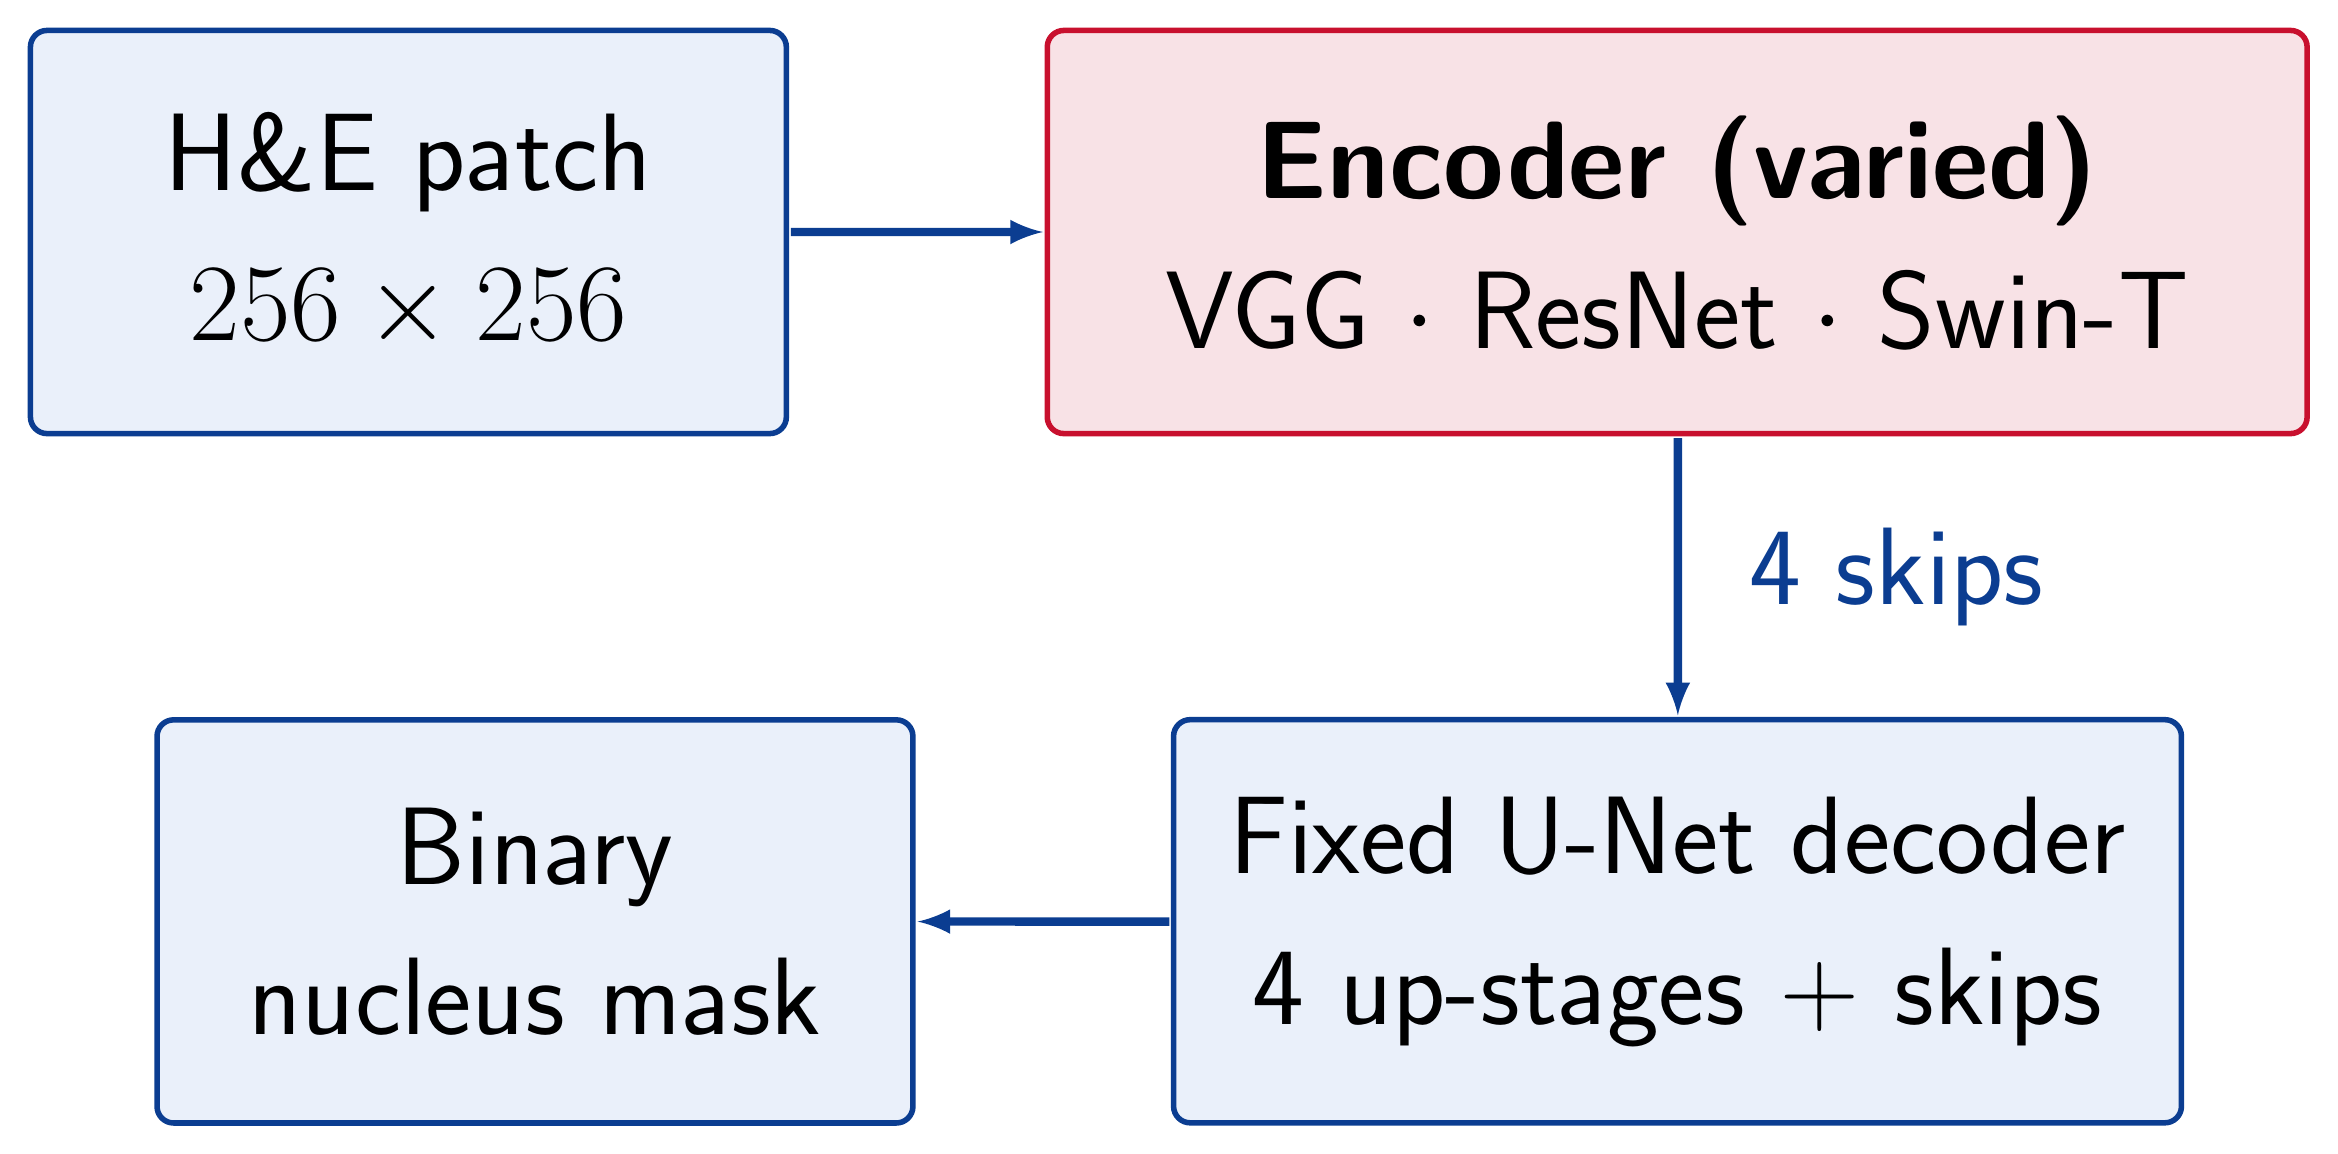
\begin{tikzpicture}[scale=1.6, transform shape, font=\fontsize{28}{34}\selectfont,
      box/.style={draw=nuBlue, line width=2pt, rounded corners=6pt, align=center,
                  minimum height=3.2cm, inner sep=10pt},
      arr/.style={-latex, line width=3pt, nuBlue}]
    \node[box, fill=paleBlue, minimum width=6cm] (in) {H\&E patch\\$256\times256$};
    \node[box, fill=nuRed!12, draw=nuRed, minimum width=10cm, right=2cm of in] (enc)
      {\textbf{Encoder (varied)}\\VGG $\cdot$ ResNet $\cdot$ Swin-T};
    \node[box, fill=paleBlue, minimum width=8cm, below=2.2cm of enc] (dec)
      {Fixed U-Net decoder\\4 up-stages + skips};
    \node[box, fill=paleBlue, minimum width=6cm, left=2cm of dec] (out) {Binary\\nucleus mask};
    \draw[arr] (in) -- (enc);
    \draw[arr] (enc) -- node[right, xshift=4mm]{4 skips} (dec);
    \draw[arr] (dec) -- (out);
  \end{tikzpicture}
  \end{tikzfigure}
  \vspace{4mm}
  Decoder, data pipeline, augmentation, optimiser and evaluation are shared; every
  encoder returns four feature maps through one interface. Results are
  \textbf{5 training seeds} on one V100, with paired 95\% CIs.

  \vspace{6mm}
  \begin{tabular}{@{}lll@{}}
    \toprule
    \textbf{Encoder} & \textbf{First skip resolution} & \textbf{Params} \\
    \midrule
    VGG (plain $3\times3$ stacks)  & $256^2$ & 34.0M \\
    ResNet (residual blocks)       & $256^2$ & 37.5M \\
    Swin-T (scratch / ImageNet)    & $64^2$ $\to$ upsampled & 86.8M \\
    \bottomrule
  \end{tabular}
}

\block{Datasets}{
  \textbf{PanNuke}: 19 tissue types, $256\times256$ patches; train fold1 (2,656 patches),
  validate fold2, test fold3.\\[4mm]
  \textbf{MoNuSeg}: \textbf{37} training slides ($1000\times1000$, 7 organs); 14 test slides
  including organs never seen in training. Tiled into $256\times256$ patches, split by slide.
}

\block{Why should CNNs win here?}{
  \begin{enumerate}
    \item \textbf{Skip resolution.} Nucleus boundaries are a few pixels wide. VGG keeps full
      resolution at its first skip; Swin's $4\times4$ tokens downsample $4\times$ at once.
    \item \textbf{Inductive bias vs data.} Attention must learn locality that convolution
      builds in, and a few thousand patches isn't enough data for that.
    \item \textbf{Input scale.} On $256^2$ patches, VGG's receptive field already spans most
      of the input by stage 4.
  \end{enumerate}
}

\block{Limitations}{
  \fontsize{26}{32}\selectfont
  5 seeds on one fixed split, so split variance isn't bounded. No learning-rate sweep, and
  the LR schedule differs between CNN and Swin. Only three encoders; at 34M parameters VGG
  isn't a truly compact model. Binary masks only, not instance separation. H\&E only.
}

% =============================================================== right column
\column{0.5}

\block{PanNuke: VGG $\approx$ ResNet $>$ Swin}{
  \begin{tikzfigure}
  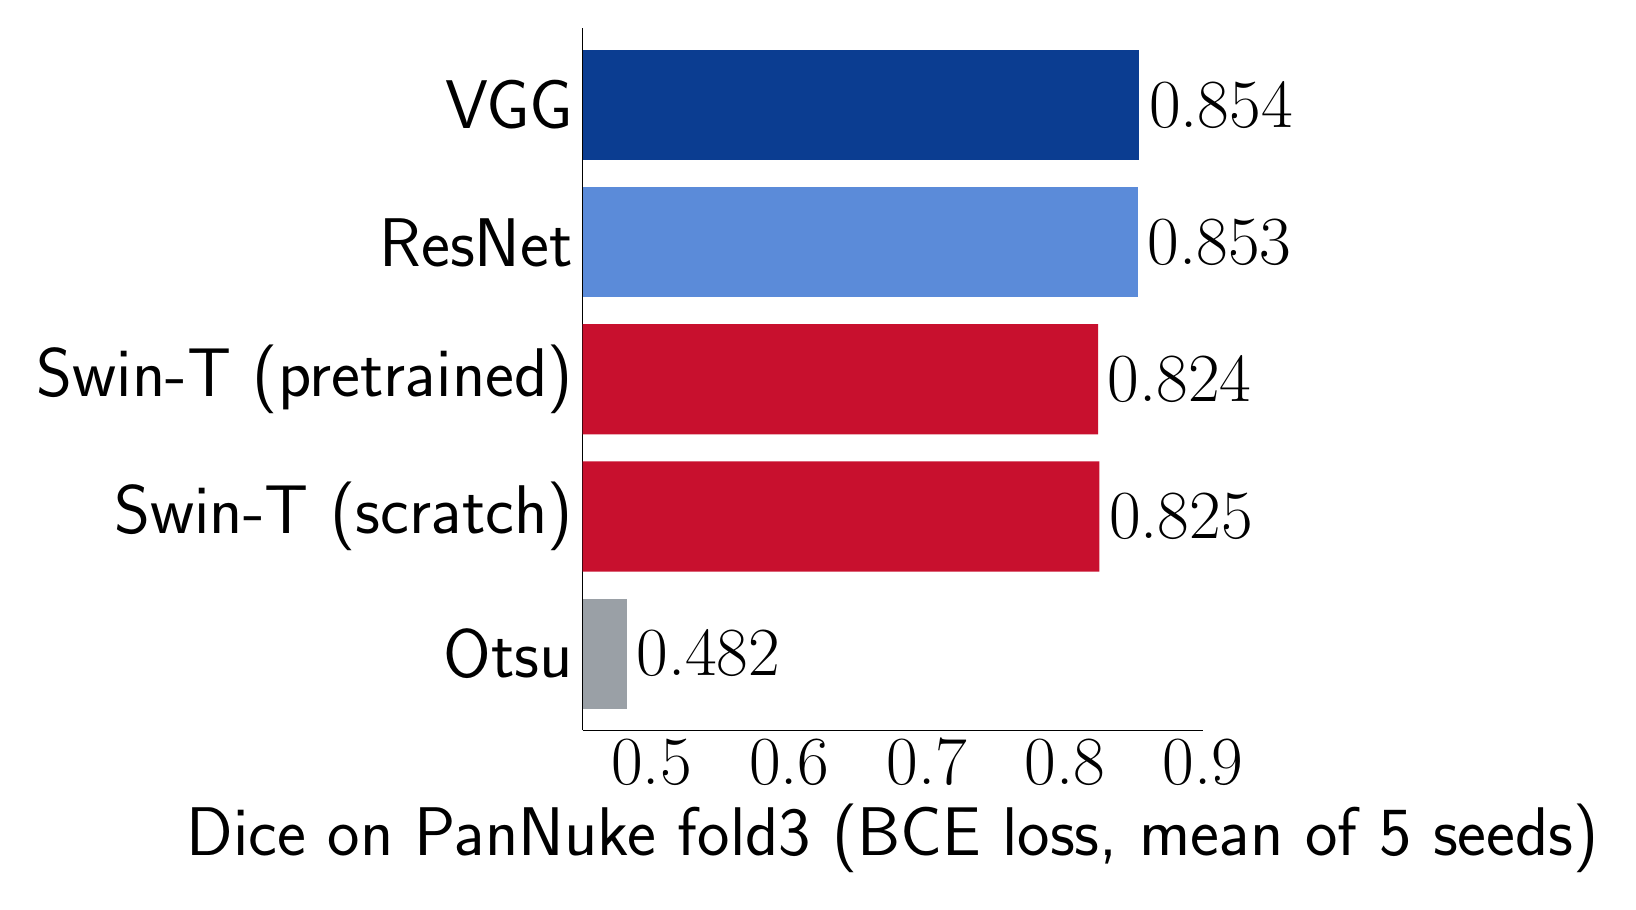
\begin{tikzpicture}
    \begin{axis}[
      xbar, bar shift=0pt, width=0.78\linewidth, height=10.5cm,
      xtick={0.5,0.6,0.7,0.8,0.9},
      xmin=0.45, xmax=0.9,
      symbolic y coords={VGG,ResNet,SwinP,SwinS,Otsu},
      yticklabels={VGG,ResNet,{Swin-T (pretrained)},{Swin-T (scratch)},Otsu},
      ytick={VGG,ResNet,SwinP,SwinS,Otsu}, y dir=reverse,
      bar width=1.4cm, enlarge y limits=0.14,
      xlabel={Dice on PanNuke fold3 (BCE loss, mean of 5 seeds)},
      tick label style={font=\fontsize{28}{32}\selectfont},
      label style={font=\fontsize{28}{32}\selectfont},
      nodes near coords, nodes near coords align={horizontal},
      every node near coord/.append style={font=\bfseries\fontsize{28}{32}\selectfont,
        /pgf/number format/fixed, /pgf/number format/precision=3,
        /pgf/number format/fixed zerofill},
      axis x line*=bottom, axis y line*=left, major tick length=0,
    ]
      \addplot[fill=vggC, draw=none] coordinates {(0.854,VGG)};
      \addplot[fill=resC, draw=none] coordinates {(0.853,ResNet)};
      \addplot[fill=swinC, draw=none] coordinates
        {(0.824,SwinP) (0.825,SwinS)};
      \addplot[fill=grayC, draw=none] coordinates {(0.482,Otsu)};
    \end{axis}
  \end{tikzpicture}
  \end{tikzfigure}
  \begin{itemize}
    \item VGG vs ResNet: $0.002$ Dice (CI $[0.001, 0.002]$), below the $0.005$ we treat as
      meaningful, so \textbf{we do not rank them}. Residual shortcuts don't help at
      four stages.
    \item VGG vs pretrained Swin: \textbf{$0.030$ Dice} (CI $[0.029, 0.031]$).
    \item ImageNet pretraining moves Swin by only $0.001$, so the gap doesn't come from
      the pretrained weights.
    \item BCE vs Dice loss: $0.854$ vs $0.856$, which is immaterial.
  \end{itemize}
}

\block{MoNuSeg: 37 training images}{
  \centering
  \begin{tabular}{@{}lccc@{}}
    \toprule
    \textbf{Model} & \textbf{Dice} & \textbf{IoU} & \textbf{Params} \\
    \midrule
    MedT (published, 30 imgs)$^\dagger$ & 0.796 & 0.662 & 1.4M \\
    Swin-T pretrained (ours) & 0.758 {\small(.007)} & 0.613 {\small(.008)} & 86.8M \\
    \textbf{\color{nuBlue}VGG (ours, scratch)} & \textbf{0.794} {\small(.011)} & \textbf{0.660} {\small(.015)} & 34.0M \\
    \bottomrule
  \end{tabular}\\[6mm]
  \raggedright
  VGG beats pretrained Swin by \textbf{0.036 Dice} (CI $[0.021, 0.052]$), a gap similar to
  PanNuke's.\\[3mm]
  {\fontsize{24}{30}\selectfont $^\dagger$A cross-paper anchor rather than a controlled
  comparison: MedT used 30 training images and $512^2$ input. We read it only as VGG
  \emph{reaching} MedT's level.\par}

  \vspace{8mm}
  \centering
  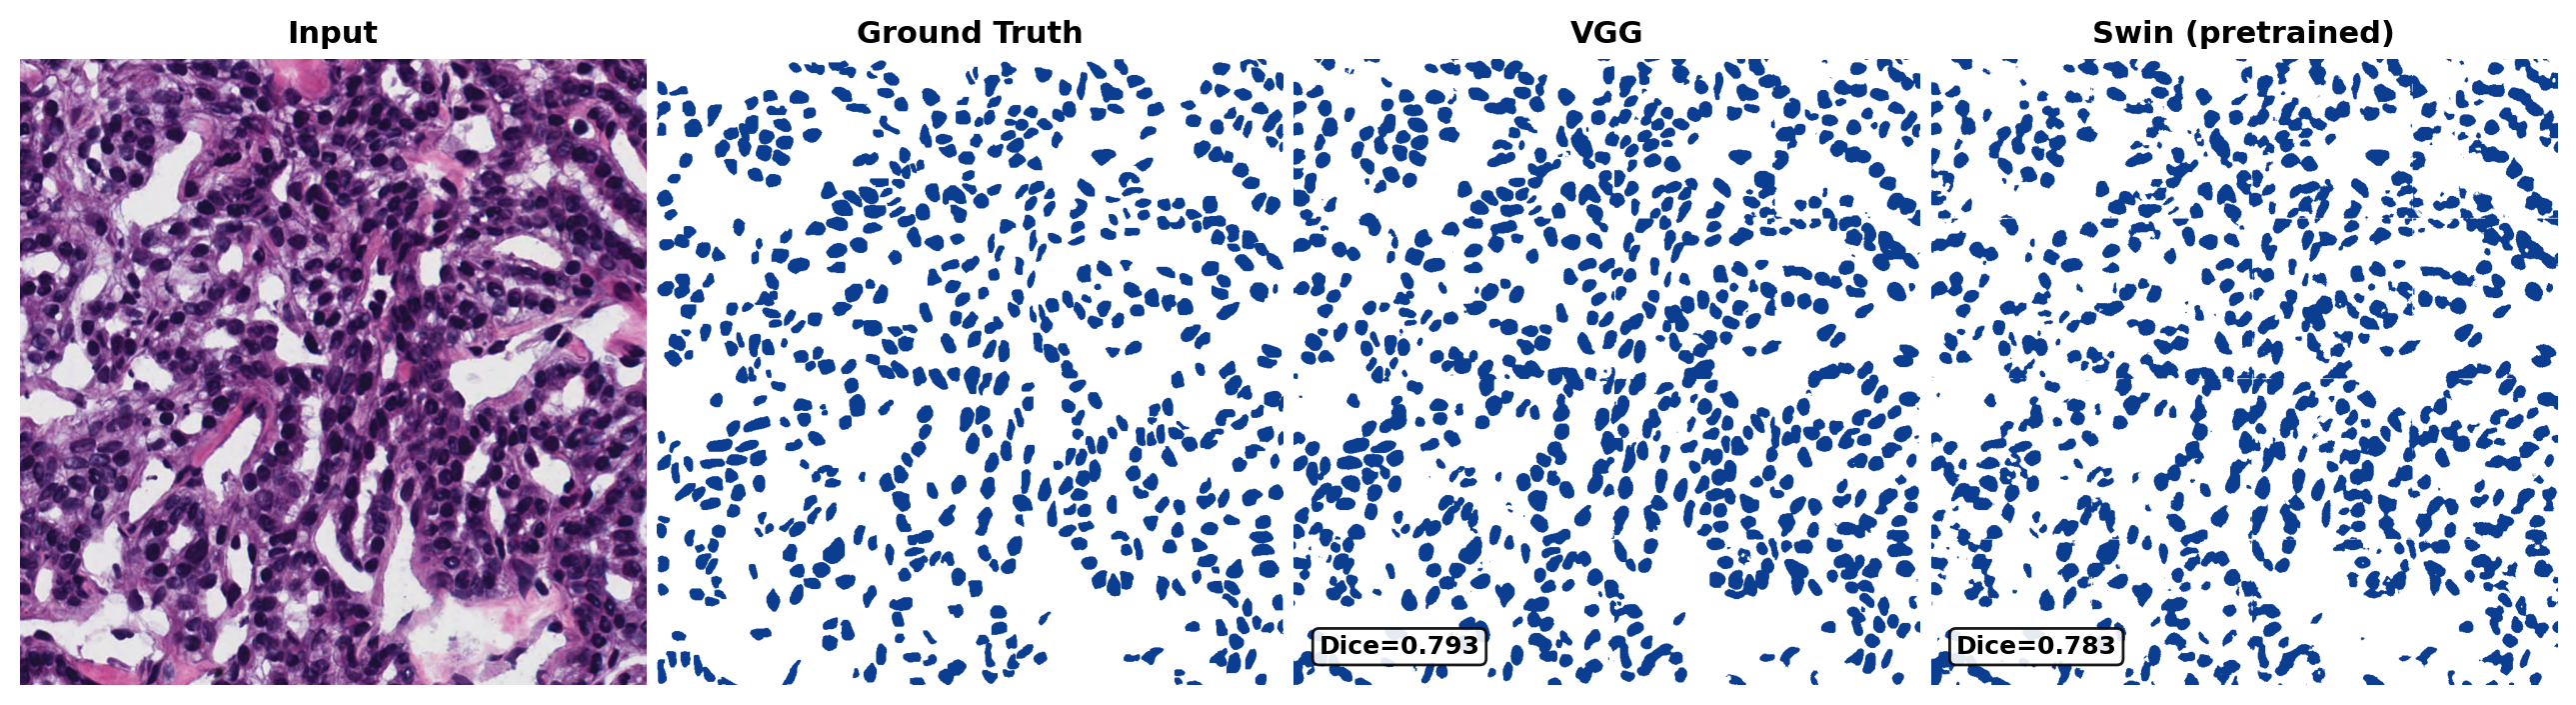
\includegraphics[width=\linewidth]{monuseg_comparison_row1_seed42_solid.png}\\[3mm]
  \raggedright
  {\fontsize{24}{30}\selectfont A dense test region, chosen for how dense it is rather
  than for the size of the gap. Swin merges neighbouring nuclei across narrow gaps
  that VGG keeps separate.\par}
}

\block{Inference cost ($256^2$, batch 1, fp32, V100)}{
  \centering
  \begin{tabular}{@{}lrrr@{}}
    \toprule
    \textbf{Model} & \textbf{Params} & \textbf{Latency} & \textbf{Peak mem.} \\
    \midrule
    \textbf{\color{nuBlue}VGG U-Net} & 34.0M & \textbf{7.1 ms} & \textbf{265 MB} \\
    ResNet U-Net & 37.5M & 9.6 ms & 277 MB \\
    Swin-T U-Net & 86.8M & 18.4 ms & 619 MB \\
    \bottomrule
  \end{tabular}\\[6mm]
  \raggedright
  \textbf{VGG is better than Swin-T on accuracy, latency and memory.} Every model we
  trained fits in 8\,GB (peak training memory: 3.6\,GiB for VGG, 5.4\,GiB for Swin).
}
\block{Next steps}{
  \fontsize{26}{32}\selectfont
  A resolution-matched Swin to separate tokenisation from encoder family; H\&E-matched
  pretraining (e.g.\ UNI); the data scale at which Swin catches up; compact
  encoders (MobileNet, ConvNeXt-T); non-H\&E stains.\\[3mm]
  \textbf{Code \& checkpoints:} github.com/Bedrockdude10/BinaryCellSegmentation
}
\end{columns}


\end{document}
